% This file was converted to LaTeX by Writer2LaTeX ver. 1.4
% see http://writer2latex.sourceforge.net for more info
\documentclass[a4paper,landscape,10pt]{article}
\usepackage[ascii]{inputenc}
\usepackage[T1]{fontenc}
\usepackage[english]{babel}
\usepackage{amsmath}
\usepackage{amssymb,amsfonts,textcomp}
\usepackage{color}
\usepackage{fancyhdr}
\usepackage[top=2.54cm,bottom=2.54cm,left=2.54cm,right=2.54cm,nohead,nofoot]{geometry}
\usepackage{array}
\usepackage{supertabular}
\usepackage{hhline}
\usepackage{hyperref}

\hypersetup{colorlinks=true, linkcolor=blue, citecolor=blue, filecolor=blue, urlcolor=blue}
\usepackage{graphicx}
\graphicspath{ {Tests_files/} }
\makeatletter
\newcommand\arraybslash{\let\\\@arraycr}
\makeatother
\raggedbottom
% Paragraph styles
\renewcommand\familydefault{\rmdefault}
\newenvironment{styleStandard}{\setlength\leftskip{0cm}\setlength\rightskip{0cm}\setlength\parindent{0cm}\setlength\parfillskip{0pt plus 1fil}\setlength\parskip{0cm plus 1pt}\writerlistparindent\writerlistleftskip\leavevmode\normalfont\normalsize\normalcolor\fontsize{11pt}{13.2pt}\selectfont\writerlistlabel\ignorespaces}{\unskip\vspace{0cm plus 1pt}\par}
% List styles
\newcommand\writerlistleftskip{}
\newcommand\writerlistparindent{}
\newcommand\writerlistlabel{}
\newcommand\writerlistremovelabel{\aftergroup\let\aftergroup\writerlistparindent\aftergroup\relax\aftergroup\let\aftergroup\writerlistlabel\aftergroup\relax}
% Footnote rule
\setlength{\skip\footins}{0.119cm}
\renewcommand\footnoterule{\vspace*{-0.018cm}\setlength\leftskip{0pt}\setlength\rightskip{0pt plus 1fil}\noindent\textcolor{black}{\rule{0.25\columnwidth}{0.018cm}}\vspace*{0.101cm}}
% Pages styles
\fancypagestyle{Standard}{\fancyhf{}
  \fancyhead[L]{}
  \fancyfoot[L]{}
  \renewcommand\headrulewidth{0pt}
  \renewcommand\footrulewidth{0pt}
  \renewcommand\thepage{\arabic{page}}
}
\pagestyle{Standard}
\setlength\tabcolsep{1mm}
\renewcommand\arraystretch{1.3}
\sloppy
\title{}
\begin{document}
\begin{flushleft}
\tablefirsthead{}
\tablehead{}
\tabletail{}
\tablelasttail{}
\begin{supertabular}{|m{1.1899999cm}|m{2.294cm}|m{2.294cm}|m{3cm}|m{1.305cm}|m{15.190001cm}|}
\hline
{\fontsize{11pt}{13.2pt}\selectfont Test number} &
{\fontsize{11pt}{13.2pt}\selectfont Description} &
{\fontsize{11pt}{13.2pt}\selectfont Data Type } &
{\fontsize{11pt}{13.2pt}\selectfont Expected Result} &
{\fontsize{11pt}{13.2pt}\selectfont Pass/Fail} &
{\fontsize{11pt}{13.2pt}\selectfont Cross Reference}\\\hline
{\fontsize{11pt}{13.2pt}\selectfont 1} &
{\fontsize{11pt}{13.2pt}\selectfont Checking that the login screen allows user to log in with their credentials.} &
{\fontsize{11pt}{13.2pt}\selectfont Typical} &
{\fontsize{11pt}{13.2pt}\selectfont System logs in using the user's data.} &
{\fontsize{11pt}{13.2pt}\selectfont Pass} &
{\fontsize{11pt}{13.2pt}\selectfont  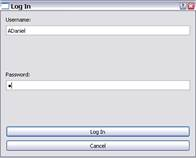
\includegraphics[width=5.186cm,height=4.18cm]{Tests-img001.jpg}
   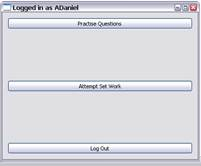
\includegraphics[width=5.318cm,height=4.392cm]{Tests-img002.jpg}
 }\\\hline
{\fontsize{11pt}{13.2pt}\selectfont 2} &
{\fontsize{11pt}{13.2pt}\selectfont Checking that the log in screen does not allow people to log in with any credentials.} &
{\fontsize{11pt}{13.2pt}\selectfont Erroneous.\newline
(Incorrect Password)} &
{\fontsize{11pt}{13.2pt}\selectfont Error message appears.\newline
(Your Username or Password is incorrect. Please try again.)} &
{\fontsize{11pt}{13.2pt}\selectfont Pass} &
{\fontsize{11pt}{13.2pt}\selectfont ~}

{\fontsize{11pt}{13.2pt}\selectfont ~}

{\fontsize{11pt}{13.2pt}\selectfont   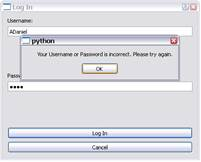
\includegraphics[width=5.318cm,height=4.286cm]{Tests-img003.jpg}
 }\\\hline
{\fontsize{11pt}{13.2pt}\selectfont 3} &
{\fontsize{11pt}{13.2pt}\selectfont Checking that the program calculates `k' correctly.} &
{\fontsize{11pt}{13.2pt}\selectfont Typical.}

{\fontsize{11pt}{13.2pt}\selectfont (6.42\^{}-1, 5.15\^{}-1, 1, 1, 4.12\^{}-4)} &
{\fontsize{11pt}{13.2pt}\selectfont Answer ~calculated using correct steps ~and being the same as on a calculator (rounded to 3sigfig).} &
{\fontsize{11pt}{13.2pt}\selectfont ~}

{\fontsize{11pt}{13.2pt}\selectfont Pass} &
{\fontsize{11pt}{13.2pt}\selectfont ~}

{\fontsize{11pt}{13.2pt}\selectfont  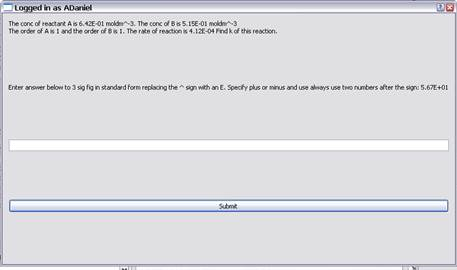
\includegraphics[width=12.091cm,height=7.144cm]{Tests-img004.jpg}
   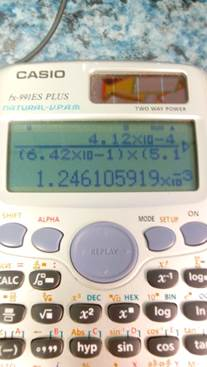
\includegraphics[width=5.477cm,height=9.71cm]{Tests-img005.jpg}
 }\\\hline
{\fontsize{11pt}{13.2pt}\selectfont 4} &
{\fontsize{11pt}{13.2pt}\selectfont Checking that the program accepts correct answers for `k' values.} &
{\fontsize{11pt}{13.2pt}\selectfont Typical} &
{\fontsize{11pt}{13.2pt}\selectfont Answer}

{\fontsize{11pt}{13.2pt}\selectfont rounded to 3 sig fig and entered in the correct format opens ``correct answer'' message box.} &
{\fontsize{11pt}{13.2pt}\selectfont ~}

{\fontsize{11pt}{13.2pt}\selectfont Pass} &
{\fontsize{11pt}{13.2pt}\selectfont ~}

{\fontsize{11pt}{13.2pt}\selectfont ~}

{\fontsize{11pt}{13.2pt}\selectfont   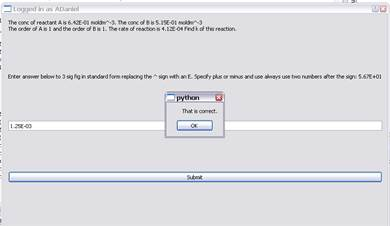
\includegraphics[width=10.319cm,height=5.98cm]{Tests-img006.jpg}
 }

{\fontsize{11pt}{13.2pt}\selectfont 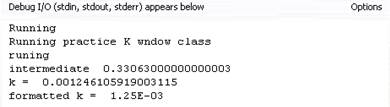
\includegraphics[width=10.319cm,height=2.831cm]{Tests-img007.jpg}
 }\\\hline
{\fontsize{11pt}{13.2pt}\selectfont 5} &
{\fontsize{11pt}{13.2pt}\selectfont Checking that the program accepts correct answers for `k' values.} &
{\fontsize{11pt}{13.2pt}\selectfont Erroneous (any incorrect answer, sdfdgido, 9.25\^{}-5).} &
{\fontsize{11pt}{13.2pt}\selectfont Answer given compared to the correct answer, then ``incorrect answer'' message box opened.} &
{\fontsize{11pt}{13.2pt}\selectfont Pass} &
{\fontsize{11pt}{13.2pt}\selectfont 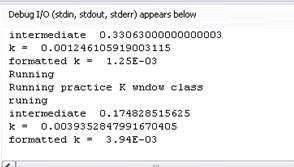
\includegraphics[width=7.779cm,height=4.419cm]{Tests-img008.jpg}\\
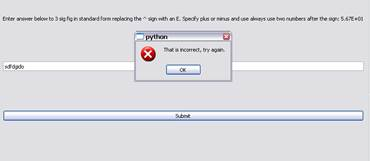
\includegraphics[width=9.79cm,height=4.26cm]{Tests-img009.jpg}
   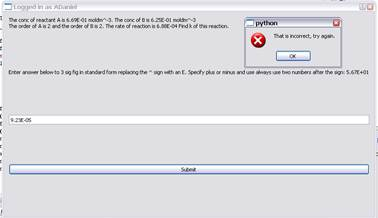
\includegraphics[width=10.001cm,height=5.766cm]{Tests-img010.jpg}
 }\\\hline
{\fontsize{11pt}{13.2pt}\selectfont 6} &
{\fontsize{11pt}{13.2pt}\selectfont That an account must have a unique username, cannot have any unfilled fields apart from middle name and that a target grade between A-U.} &
{\fontsize{11pt}{13.2pt}\selectfont Typical}

{\fontsize{11pt}{13.2pt}\selectfont (Student,Jack,William,Montfort,salmon,JMontfort, 12EJP, A)} &
{\fontsize{11pt}{13.2pt}\selectfont Student account allowed to be made, ``new student created'' message box opened.} &
{\fontsize{11pt}{13.2pt}\selectfont Pass} &
{\fontsize{11pt}{13.2pt}\selectfont ~}

{\fontsize{11pt}{13.2pt}\selectfont   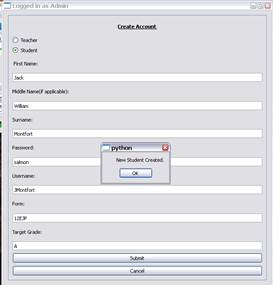
\includegraphics[width=7.223cm,height=7.541cm]{Tests-img011.jpg}
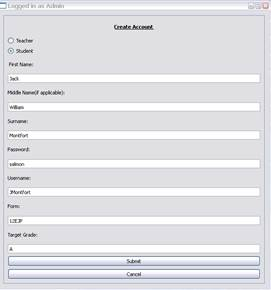
\includegraphics[width=7.17cm,height=7.671cm]{Tests-img012.jpg}
 }\\\hline
{\fontsize{11pt}{13.2pt}\selectfont 7} &
{\fontsize{11pt}{13.2pt}\selectfont Testing that accounts are saved when created.} &
{\fontsize{11pt}{13.2pt}\selectfont Data entered in last test.} &
{\fontsize{11pt}{13.2pt}\selectfont Correct student account details printed out.} &
{\fontsize{11pt}{13.2pt}\selectfont Pass} &
{\fontsize{11pt}{13.2pt}\selectfont  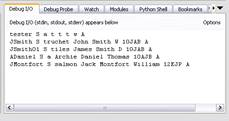
\includegraphics[width=6.057cm,height=3.201cm]{Tests-img013.jpg}
 }\\\hline
{\fontsize{11pt}{13.2pt}\selectfont 8} &
{\fontsize{11pt}{13.2pt}\selectfont Checking that only valid information can be input into the fields.} &
{\fontsize{11pt}{13.2pt}\selectfont Erroneous}

{\fontsize{11pt}{13.2pt}\selectfont (Target grade correct as this is picked up, but the rest are not).} &
{\fontsize{11pt}{13.2pt}\selectfont Student account not made, error message displayed.} &
{\fontsize{11pt}{13.2pt}\selectfont Pass} &
{\fontsize{11pt}{13.2pt}\selectfont  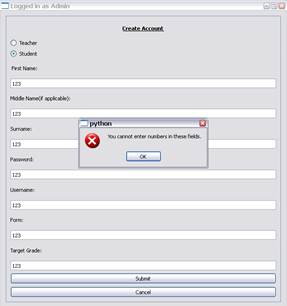
\includegraphics[width=7.594cm,height=8.096cm]{Tests-img014.jpg}
 }\\\hline
{\fontsize{11pt}{13.2pt}\selectfont 9} &
{\fontsize{11pt}{13.2pt}\selectfont Clicking the ``Practise Questions'' button opens the ``Practise Questions'' window.} &
{\fontsize{11pt}{13.2pt}\selectfont Typical}

{\fontsize{11pt}{13.2pt}\selectfont (clicking the correct button)} &
{\fontsize{11pt}{13.2pt}\selectfont Practise questions window opens.} &
{\fontsize{11pt}{13.2pt}\selectfont Pass} &
{\fontsize{11pt}{13.2pt}\selectfont   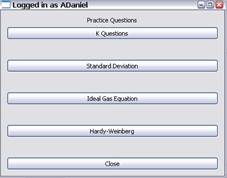
\includegraphics[width=6.006cm,height=4.71cm]{Tests-img015.jpg}
 }\\\hline
{\fontsize{11pt}{13.2pt}\selectfont 10} &
{\fontsize{11pt}{13.2pt}\selectfont That total population has to be bigger than the amount of heterozygous individuals when making a Hardy-Weinberg question.} &
{\fontsize{11pt}{13.2pt}\selectfont Erroneous}

{\fontsize{11pt}{13.2pt}\selectfont (Larger homozygous recessive,300, than total population , 32)} &
{\fontsize{11pt}{13.2pt}\selectfont Question is not allowed to be created, error message opens.} &
{\fontsize{11pt}{13.2pt}\selectfont Pass} &
{\fontsize{11pt}{13.2pt}\selectfont  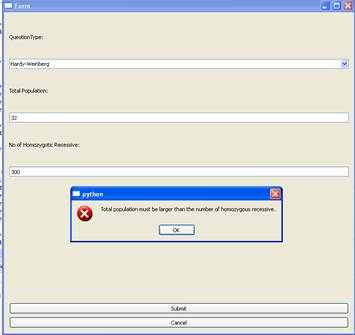
\includegraphics[width=9.393cm,height=8.864cm]{Tests-img016.jpg}
 }\\\hline
{\fontsize{11pt}{13.2pt}\selectfont 11} &
{\fontsize{11pt}{13.2pt}\selectfont That total population has to be bigger than the amount of heterozygous individuals when making a Hardy-Weinberg question.} &
{\fontsize{11pt}{13.2pt}\selectfont Typical (total pop 32, no of homozygous recessive 10)} &
{\fontsize{11pt}{13.2pt}\selectfont Question allowed to be created, confirmation message box.} &
{\fontsize{11pt}{13.2pt}\selectfont Pass} &
{\fontsize{11pt}{13.2pt}\selectfont ~}

{\fontsize{11pt}{13.2pt}\selectfont   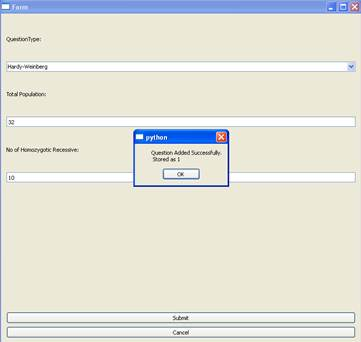
\includegraphics[width=9.551cm,height=9.049cm]{Tests-img017.jpg}
 }\\\hline
{\fontsize{11pt}{13.2pt}\selectfont 12} &
{\fontsize{11pt}{13.2pt}\selectfont That questions are stored correctly in questions.pickle} &
{\fontsize{11pt}{13.2pt}\selectfont Data from last test} &
{\fontsize{11pt}{13.2pt}\selectfont Correct question details printed from pickle.} &
{\fontsize{11pt}{13.2pt}\selectfont Pass} &
{\fontsize{11pt}{13.2pt}\selectfont ~}

{\fontsize{11pt}{13.2pt}\selectfont  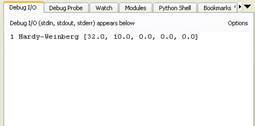
\includegraphics[width=6.747cm,height=3.334cm]{Tests-img018.jpg}
 }

{\fontsize{11pt}{13.2pt}\selectfont ~}\\\hline
{\fontsize{11pt}{13.2pt}\selectfont 13} &
{\fontsize{11pt}{13.2pt}\selectfont Testing that questions can be added to a QSet, that duplicate questions can't be added and that QSets can be saved if they fit the correct criteria.} &
{\fontsize{11pt}{13.2pt}\selectfont Typical(1 : Hardy-Weinberg, 2 : Rate Constant)} &
{\fontsize{11pt}{13.2pt}\selectfont Selected fields move to the ``New Set'' box, questions cannot be moved to the ``New Set'' box if they are already in the ``New Set'' box. A message box opens saying that a question set has been .} &
{\fontsize{11pt}{13.2pt}\selectfont Pass} &
{\fontsize{11pt}{13.2pt}\selectfont   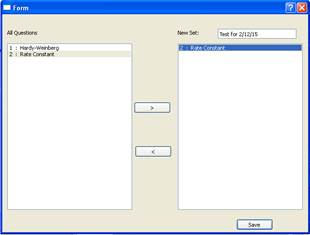
\includegraphics[width=8.202cm,height=6.218cm]{Tests-img019.jpg}
  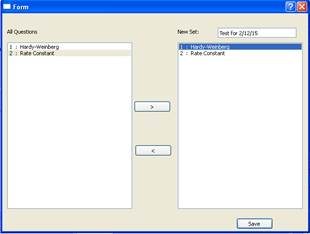
\includegraphics[width=8.202cm,height=6.191cm]{Tests-img020.jpg}
  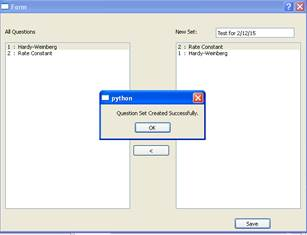
\includegraphics[width=8.123cm,height=6.218cm]{Tests-img021.jpg}
 }\\\hline
{\fontsize{11pt}{13.2pt}\selectfont 14} &
{\fontsize{11pt}{13.2pt}\selectfont Testing that a QSet is saved.} &
{\fontsize{11pt}{13.2pt}\selectfont Typical(1 : Hardy-Weinberg, 2 : Rate Constant)} &
{\fontsize{11pt}{13.2pt}\selectfont Correct QSet details printed out.} &
{\fontsize{11pt}{13.2pt}\selectfont Pass} &
{\fontsize{11pt}{13.2pt}\selectfont ~}

{\fontsize{11pt}{13.2pt}\selectfont  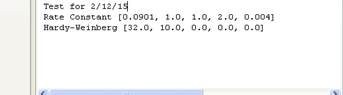
\includegraphics[width=9.075cm,height=2.514cm]{Tests-img022.jpg}
 }\\\hline
{\fontsize{11pt}{13.2pt}\selectfont 15} &
{\fontsize{11pt}{13.2pt}\selectfont Test that a QSet must have a name to be created} &
{\fontsize{11pt}{13.2pt}\selectfont No name entered.} &
{\fontsize{11pt}{13.2pt}\selectfont Error message opens and QSet is not saved.} &
{\fontsize{11pt}{13.2pt}\selectfont Pass} &
{\fontsize{11pt}{13.2pt}\selectfont   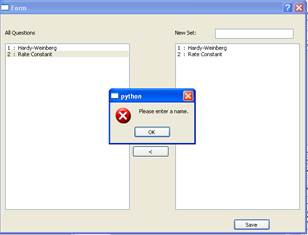
\includegraphics[width=8.149cm,height=6.218cm]{Tests-img023.jpg}
 ~~~~~~~~~~~~~~~~~ }\\\hline
{\fontsize{11pt}{13.2pt}\selectfont 16} &
{\fontsize{11pt}{13.2pt}\selectfont Test that a QSet must have questions in it to be created.} &
{\fontsize{11pt}{13.2pt}\selectfont No questions put in ``New Set'' box} &
{\fontsize{11pt}{13.2pt}\selectfont Error message opens and QSet is not saved.} &
{\fontsize{11pt}{13.2pt}\selectfont Pass} &
{\fontsize{11pt}{13.2pt}\selectfont   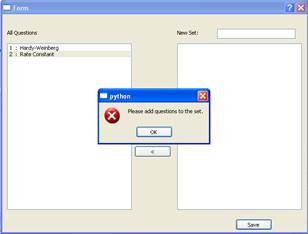
\includegraphics[width=8.149cm,height=6.191cm]{Tests-img024.jpg}
 }\\\hline
{\fontsize{11pt}{13.2pt}\selectfont 17} &
{\fontsize{11pt}{13.2pt}\selectfont ~} &
{\fontsize{11pt}{13.2pt}\selectfont ~} &
{\fontsize{11pt}{13.2pt}\selectfont ~} &
{\fontsize{11pt}{13.2pt}\selectfont ~} &
{\fontsize{11pt}{13.2pt}\selectfont ~}\\\hline
\end{supertabular}
\end{flushleft}

\bigskip

\begin{styleStandard}
~
\end{styleStandard}

\begin{styleStandard}
~
\end{styleStandard}

\begin{styleStandard}
~
\end{styleStandard}

\begin{styleStandard}
~
\end{styleStandard}

\begin{styleStandard}
~
\end{styleStandard}

\begin{styleStandard}
\textit{~lol}
\end{styleStandard}

\begin{styleStandard}
\textit{~}
\end{styleStandard}

\begin{styleStandard}
~
\end{styleStandard}

\begin{styleStandard}
\textit{~}
\end{styleStandard}

\begin{styleStandard}
~
\end{styleStandard}

\begin{styleStandard}
~
\end{styleStandard}

\begin{styleStandard}
~
\end{styleStandard}

\begin{styleStandard}
~
\end{styleStandard}

\begin{styleStandard}
~
\end{styleStandard}

\begin{styleStandard}
~
\end{styleStandard}

\begin{styleStandard}
~
\end{styleStandard}

\begin{styleStandard}
~
\end{styleStandard}

\begin{styleStandard}
~
\end{styleStandard}

\begin{styleStandard}
~
\end{styleStandard}

\begin{styleStandard}
~
\end{styleStandard}

\begin{styleStandard}
~
\end{styleStandard}

\begin{styleStandard}
~
\end{styleStandard}

\begin{styleStandard}
~
\end{styleStandard}


\bigskip
\end{document}
